\begin{figure}
    \centering
    %\tikzstyle{block} = [rectangle, rounded corners, text=black, text centered, draw=black, minimum height=.3in]
    \tikzstyle{block} = [rectangle, rounded corners, text=black, text centered, draw=black,font=\footnotesize, minimum height=.21in, minimum width=.65in]
    \tikzstyle{line} = [-latex,draw=black,line width=.4]
    \tikzstyle{line2} = [latex-latex,draw=black,line width=.4]
    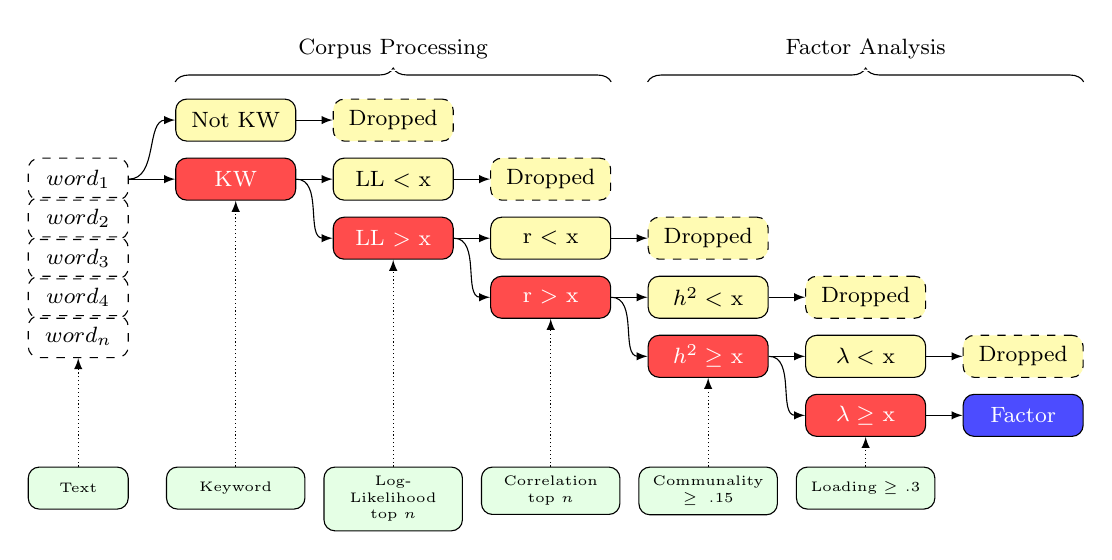
\begin{tikzpicture}
        \node[block,text=black, minimum width=.5in, dashed] (word1) at (10,11) {$word_1$};
        \node[block,text=black, minimum width=.5in, dashed] (word2) at (10,10.5) {$word_2$};
        \node[block,text=black, minimum width=.5in, dashed] (word3) at (10,10) {$word_3$};
        \node[block,text=black, minimum width=.5in, dashed] (word4) at (10,9.5) {$word_4$};
        \node[block,text=black, minimum width=.5in, dashed] (wordn) at (10,9) {$word_n$};
        \node[block,text=black, fill=yellow!30, minimum width=.6in] (notKW) at (12,11.75) {Not KW};
        \node[block,text=white, fill=red!70, minimum width=.6in] (KW) at (12,11) {KW};
        \node[block,text=black, minimum width=.6in, dashed, fill=yellow!30] (dropped1) at (14,11.75) {Dropped};
        \node[block,text=black, fill=yellow!30, minimum width=.6in] (notLL) at (14,11) {LL $<$ x};
        \node[block,text=white, fill=red!70, minimum width=.6in] (LL) at (14,10.25) {LL $>$ x};
        \node[block,text=black, minimum width=.6in, dashed, fill=yellow!30] (dropped2) at (16,11) {Dropped};
        \node[block,text=black, fill=yellow!30, minimum width=.6in] (notR) at (16,10.25) {r $<$ x};
        \node[block,text=white, fill=red!70, minimum width=.6in] (R) at (16,9.5) {r $>$ x};
        %\node[block,text=white, fill=red!70, minimum width=.6in] (R) at (16,9.5) {$S_r 1\dots n]_r$};
        \node[block,text=black, minimum width=.6in, dashed, fill=yellow!30] (dropped3) at (18,10.25) {Dropped};
        \node[block,text=black, fill=yellow!30,minimum width=.6in] (notH) at (18,9.5) {$h^2 <$ x};
        \node[block,text=white, fill=red!70,minimum width=.6in] (H) at (18,8.75) {$h^2 \geq$ x};
        \node[block,text=black, minimum width=.6in, dashed, fill=yellow!30] (dropped4) at (20,9.5) {Dropped};
        \node[block,text=black, fill=yellow!30, minimum width=.6in] (notloading) at (20,8.75) {$\lambda <$ x};
        \node[block,text=white, fill=red!70,minimum width=.6in] (loading) at (20,8) {$\lambda \geq$ x};
        \node[block,text=black, minimum width=.6in, dashed, fill=yellow!30] (dropped5) at (22,8.75) {Dropped};
        \node[block,text=white, fill=blue!70,minimum width=.6in] (factor) at (22,8) {Factor};
        \draw[line] (word1) to [in=180,out=0] (notKW);
        \draw[line] (word1) to [in=180,out=0] (KW);
        \draw[line] (KW) to [in=180,out=0] (notLL);
        \draw[line] (KW) to [in=180,out=0] (LL);
        \draw[line] (LL) to [in=180,out=0] (notR);
        \draw[line] (LL) to [in=180,out=0] (R);
        \draw[line] (R) to [in=180,out=0] (notH);
        \draw[line] (R) to [in=180,out=0] (H);
        \draw[line] (H) to [in=180,out=0] (notloading);
        \draw[line] (H) to [in=180,out=0] (loading);
        \draw[line] (loading) to [in=180,out=0] (factor);
        \draw[line] (notKW) to [in=180,out=0] (dropped1);
        \draw[line] (notLL) to [in=180,out=0] (dropped2);
        \draw[line] (notR) to [in=180,out=0] (dropped3);
        \draw[line] (notH) to [in=180,out=0] (dropped4);
        \draw[line] (notloading) to [in=180,out=0] (dropped5);
        \node[block,text=black, fill=green!10, minimum width=.5in, anchor=north, font=\tiny] (text) at (10,7.35) {Text};
        \node[block,text=black, fill=green!10, minimum width=.6in, text width=.6in, anchor=north, font=\tiny] (keyword) at (12,7.35) {Keyword};
        \node[block,text=black, fill=green!10, minimum width=.6in, text width=.6in, anchor=north, font=\tiny] (log) at (14,7.35) {Log-Likelihood top $n$};
        \node[block,text=black, fill=green!10, minimum width=.6in, text width=.6in, anchor=north, font=\tiny] (correlation) at (16,7.35) {Correlation top $n$};
        \node[block,text=black, fill=green!10, minimum width=.6in, text width=.6in, anchor=north, font=\tiny] (comm) at (18,7.35) {Com\-mun\-al\-i\-ty $\geq .15$};
        \node[block,text=black, fill=green!10, minimum width=.6in, text width=.6in, anchor=north, font=\tiny] (loadingbottom) at (20,7.35) {Loading $\geq .3$};
        \draw[line, densely dotted] (text) to (wordn);
        \draw[line, densely dotted] (keyword) to (KW);
        \draw[line, densely dotted] (log) to (LL);
        \draw[line, densely dotted] (correlation) to (R);
        \draw[line, densely dotted] (comm) to (H);
        \draw[line, densely dotted] (loadingbottom) to (loading);
        %\draw[decorate,decoration={brace,amplitude=5pt,raise=6pt,mirror}] (collocateL4.south west) -- (collocateR4.south east);
        \node[block, draw=white, minimum width=.6in] (blank1) at (16,11.75) {};
        \node[block, draw=white, minimum width=.6in] (blank2) at (18,11.75) {};
        \node[block, draw=white, minimum width=.6in] (blank3) at (22,11.75) {};
        \draw[decorate,decoration={brace,amplitude=5pt,raise=6pt}] (notKW.north west) -- (blank1.north east);
        \draw[decorate,decoration={brace,amplitude=5pt,raise=6pt}] (blank2.north west) -- (blank3.north east);
        \node[block, draw=white, minimum width=.6in] (processing) at (14,12.65) {Corpus Processing};
        \node[block, draw=white, minimum width=.6in] (processing) at (20,12.65) {Factor Analysis};
    \end{tikzpicture}
    \caption{From text to factor}
    \label{fig:from_text_to_factor}
\end{figure}
